\ifx\pdfminorversion\undefined\else\pdfminorversion=7\fi
\documentclass[pdflatex,sn-basic,Numbered,iicol]{sn-jnl}

\usepackage{graphicx}%
\usepackage{multirow}%
\usepackage{tabularx}%
\usepackage{array}%
\usepackage{amsmath,amssymb,amsfonts}%
\usepackage[title]{appendix}%
\usepackage{xcolor}%
\usepackage{textcomp}%
\usepackage{booktabs}%
\usepackage{url}%

\graphicspath{{figures/}}

\raggedbottom

\newcounter{algorithm}
\newenvironment{algorithmblock}[1]{%
  \refstepcounter{algorithm}%
  \par\smallskip
  \noindent\begin{minipage}{\linewidth}
  \small
  \hrule
  \vspace{0.45em}
  \noindent\textbf{Algorithm~\thealgorithm. #1}\par
  \vspace{0.35em}
}{%
  \vspace{0.35em}
  \hrule
  \end{minipage}
  \par\smallskip
}

\title[Budgeted Preprocessing Selection for Vietnamese Administrative OCR]{Budgeted Page-Level Preprocessing Selection for Vietnamese Administrative OCR: A Controlled Comparison of Learned, Retrieval-Based, and Static Shortlists}

\author[1]{\fnm{Cong Thanh} \sur{Bui}}\email{congthanhttmt@gmail.com}
\equalcont{These authors contributed equally to this work and share first authorship.}

\author*[1]{\fnm{Van Anh} \sur{Nguyen}}\email{nguyenanhbh14@gmail.com}
\equalcont{These authors contributed equally to this work and share first authorship.}

\author[1]{\fnm{The Hung} \sur{Nguyen}}\email{hungnguyenthe1211@gmail.com}

\author[1]{\fnm{Anh Tu} \sur{Nguyen}}\email{nguyenanhtu789@gmail.com}

\author[1]{\fnm{Thi Quynh} \sur{Le}}\email{lequynh.k51.ktqs@gmail.com}

\author[1]{\fnm{Thi Linh} \sur{Lai}}\email{linhlai1605@gmail.com}

\author[1]{\fnm{Trung Dung} \sur{Nguyen}}\email{ntdtoanud2011@gmail.com}

\affil[1]{\orgname{National Laboratory for Securing Information (NLSI), Ministry of National Defence}, \orgaddress{\city{Hanoi}, \country{Vietnam}}}

\abstract{\textbf{Purpose:} We study page-level preprocessing selection for administrative-document OCR under a limited OCR-call budget. \textbf{Methods:} A stratified five-parameter design produces 50 configurations. Recognizer-specific CER regressors rank them using OCR-free page features and configuration parameters. Nested GroupKFold compares surrogate, nearest-neighbor transfer (NN-K), FixedTopK, and random shortlists on 300 Vietnamese administrative first pages, with and without contour suppression, and 626 SROIE receipts. An oracle-free selector chooses one output from the surrogate top-3. \textbf{Results:} Surrogate and NN-K significantly outperform random shortlists across all recognizers, settings, and budgets. FixedTopK is competitive on Vietnamese data, whereas the surrogate significantly outperforms it in all eight SROIE comparisons. Headroom correlates with the other three policies' FixedTopK-relative gains; Random's correlation exceeds Surrogate's in 30/32 cases, supporting a policy-agnostic interpretation. The selector yields lower mean CER than the static single-best configuration (FixedBest) in all eight settings; six tests have unadjusted $p<0.05$, and three remain significant after Holm correction. \textbf{Conclusion:} No shortlist policy is uniformly best. Page-conditioned shortlists outperform random sampling; the selector requires no reference text at inference time.}

\keywords{document OCR, preprocessing selection, algorithm selection, surrogate-based ranking, nearest-neighbor transfer, oracle-free output selection}

\begin{document}
\maketitle

\section{Introduction}
\label{sec:introduction}

Optical character recognition (OCR) on administrative documents remains sensitive to seemingly low-level image preparation choices. In Vietnamese administrative documents, two issues are especially prominent. First, stamps, decorative headers, and logos can cause a detector to generate false or low-quality text crops. Second, the effectiveness of denoising, contrast enhancement, brightness correction, and sharpening varies substantially across pages, making any single static preprocessing recipe unreliable.

The straightforward solution to the second issue is exhaustive per-image search over preprocessing combinations, but this is expensive because every candidate requires a full OCR pass. This creates a practical ranking problem: can a model trained once on previously observed documents identify a small shortlist of promising preprocessing configurations for a new page?

This paper studies that question in a page-level OCR pipeline built around PaddleOCR detection and three different recognizers. The proposed framework treats preprocessing choice as budgeted page-conditioned shortlist selection over a fixed candidate pool. A stratified design over a five-parameter preprocessing space is used to construct a fixed 50-candidate pool; each candidate is then evaluated with OCR to obtain observed CER values. Page-level features are extracted once from each page, and learned surrogate, retrieval-based, and static shortlist policies are compared under identical fixed-budget evaluation.

Two questions determine whether this formulation is practically useful. First, how do learned surrogate ranking, retrieval from visually similar pages, and a static shortlist compare under the same OCR-call budget? Second, can a promising shortlist be reduced to one output without using reference text at inference time? We address the first question through nested, page-grouped comparisons against Random K and FixedTopK, and the second through a nested oracle-free top-3 selector. We also analyze the per-page FixedTopK-to-oracle headroom as a retrospective property of the candidate pool. Because headroom and any FixedTopK-relative policy advantage share the FixedTopK term, we include Random and NN-K controls and do not interpret their correlation as evidence specific to learned ranking.

The paper makes the following contributions:
\begin{enumerate}
    \item It formulates page-level OCR preprocessing as a budgeted shortlist-selection problem over a fixed candidate pool and evaluates it across recognizers, preprocessing conditions, and a second document domain.
    \item It provides a controlled nested GroupKFold comparison of cross-instance surrogate ranking, nearest-neighbor transfer, static FixedTopK, and random shortlist policies under identical OCR-call budgets.
    \item It evaluates a nested oracle-free top-3 output selector that selects one OCR result from a surrogate shortlist without reference text at inference time.
    \item It provides controlled diagnostics of FixedTopK-to-sampled-oracle headroom using shared-baseline and direct policy-to-policy controls, separating retrospective improvement potential from policy-specific evidence.
\end{enumerate}

This article is related to an earlier conference paper by the authors on hybrid OCR for Vietnamese administrative documents \cite{Thanh2025HOCR}. The earlier work focused on an end-to-end OCR pipeline that combined PaddleOCR detection, VietOCR recognition, stamp handling, and language-model-based post-processing. In contrast, the present article addresses a different methodological question: how page-level preprocessing candidates can be prioritized under a fixed OCR budget. Compared with the conference paper, the present study introduces a fixed candidate-pool formulation, recognizer-specific surrogate modeling, static and retrieval-based shortlist baselines, nested GroupKFold evaluation, paired statistical comparisons, oracle-free top-3 output selection, and evaluation on the SROIE receipt dataset.

The paper is organized as follows. Section~\ref{sec:related_work} reviews related work. Section~\ref{sec:dataset_problem} describes the datasets and task definition. Section~\ref{sec:method} formalizes the proposed method. Section~\ref{sec:experimental_setup} details the experimental setup. Section~\ref{sec:results} reports the main results. Section~\ref{sec:discussion} discusses interpretation and practical implications. Section~\ref{sec:limitations} outlines limitations, and Section~\ref{sec:conclusion} concludes.

\section{Related Work}
\label{sec:related_work}

\subsection{OCR Systems and Document Preprocessing}

Modern modular OCR pipelines, including PaddleOCR/PP-OCR, separate detection from recognition, with detected text regions cropped before recognition \cite{du2020ppocr,li2022ppocrv3}. Our pipeline follows this structure with PaddleOCR detection and three alternative recognizers based on different design assumptions: Tesseract \cite{smith2007tesseract}, EasyOCR \cite{easyocrsoftware}, and the Vietnamese-specific VietOCR \cite{vietocrsoftware}. Vietnamese document analysis and OCR is an active application area facing complex diacritics, limited annotated data, and real-world document variation \cite{le2025vietnamesedar}, with representative work spanning scene-text recognition and the VinText benchmark \cite{nguyen2021vintext}, administrative-document digitization \cite{nguyen2021digitalization}, and MC-OCR receipt recognition \cite{vu2021mcocr}. Against this background, this paper studies adaptive page-level preprocessing selection as an orthogonal axis to recognizer choice; the recognizers themselves remain unmodified.

Document image preprocessing has a long history in OCR. Global thresholding such as Otsu's method \cite{otsu1979threshold} and local/adaptive methods such as Sauvola and Pietik\"{a}inen \cite{sauvola2000adaptive} are canonical baselines, with DIBCO-style evaluations established as benchmarks for historical and degraded documents \cite{gatos2011dibco}. Beyond binarization, OCR pipelines often use photometric enhancement and denoising operations such as contrast-limited adaptive histogram equalization (CLAHE) \cite{zuiderveld1994clahe}, bilateral filtering \cite{tomasi1998bilateral}, gamma correction, and unsharp masking; these directly motivate the parameter space evaluated here. Recent learned restoration methods, including DE-GAN \cite{souibgui2022degan} and DocEnTr \cite{souibgui2022docentr}, learn image-to-image enhancement transforms and are complementary to our setting, which instead learns a cross-instance surrogate that ranks lightweight preprocessing parameter settings by downstream OCR CER. Administrative documents also contain artifacts such as stamps, decorative headers, and watermarks; this motivates the contour-suppression setting evaluated here, while the main contribution remains budgeted prioritization of preprocessing candidates rather than artifact removal.

\subsection{Algorithm Selection, Meta-Learning, and Surrogate Optimization}

Surrogate and sequential model-based optimization methods are also relevant to our setting. Methods such as SMAC \cite{hutter2011smac}, Bayesian optimization frameworks \cite{snoek2012practical}, and TPE-based sequential optimization \cite{bergstra2011algorithms} guide a sequential optimization run: configurations are evaluated iteratively, and the search model or distribution is updated from observations collected during that run. In standard formulations, this process is optimized for the current task rather than reused unchanged to rank a fixed pool on unseen document pages. In contrast, our surrogate is trained once across many document pages and reused at inference to rank preprocessing candidates for a new page without per-image OCR feedback.

Our data collection strategy is also closer to design-of-experiments than to iterative Bayesian optimization. Space-filling designs such as Latin hypercube sampling \cite{mckay1979lhs} are useful for broadly covering the preprocessing parameter space during offline data collection.

Closer to adaptive preprocessing, Garg and Chaudhury \cite{garg2016adaptive} studied automatic selection of document-image enhancement parameters using image-quality assessment and expected recognition accuracy within an EM-based optimization framework. Vats et al. \cite{vats2017bayesian} applied Bayesian optimization to hyperparameter selection in document image binarization, and Singh et al. \cite{singh2018surrogate} learned surrogate models for document image quality metrics to support automated document image processing. These studies support the relevance of adaptive parameter selection and surrogate modeling in document preprocessing. However, the studies by Garg and Chaudhury and by Vats et al. focus on parameter optimization and binarization, whereas Singh et al. use cross-image surrogate modeling for document-image quality metric estimation rather than OCR-CER-based shortlist ranking.

\subsection{Positioning of This Work}

This work sits at the intersection of OCR preprocessing, algorithm selection, and surrogate modeling. Unlike OCR-engine papers, it does not introduce a new detector or recognizer. Unlike classical preprocessing studies, it does not propose one fixed filter or binarization rule. Unlike standard Bayesian optimization, it does not perform iterative per-image search. Compared with prior automatic preprocessing parameter-selection work, our formulation shifts the problem from estimating a single optimal preprocessing setting to selecting a small candidate shortlist under a fixed OCR budget. This enables direct comparison of static, retrieval-based, and learned shortlist policies, where the key requirement is not exact CER prediction but reliable prioritization of candidate preprocessing settings.

Three empirical findings structure the paper's contributions. First, page-conditioned shortlist construction (surrogate and NN-K) reliably outperforms random shortlist selection in all evaluated comparisons (24/24 Vietnamese and 8/8 SROIE) under identical OCR-call budgets, even with moderate surrogate $R^2$. FixedTopK is stronger than Random K and remains highly competitive on the Vietnamese data, so the learned, retrieval-based, and static policies form a setting-dependent ordering rather than a single uniformly dominant policy. Second, the apparent association between the gap from FixedTopK to the sampled-pool oracle and each policy's advantage over FixedTopK is policy-agnostic: the same coupled relationship appears for Random and NN-K, while direct policy-to-policy controls do not support an interpretation specific to learned ranking. Third, a nested oracle-free top-3 selector recovers part of the shortlist gain without reference text at inference time and has lower mean CER than FixedBest in all eight settings; six paired tests have unadjusted $p<0.05$, and three remain significant after Holm correction across the eight comparisons. To our knowledge, this specific problem formulation---budgeted page-conditioned shortlist ranking for OCR preprocessing, with controlled comparison of learned, retrieval-based, static, and random policies plus nested oracle-free output selection---has not been explicitly studied in the OCR preprocessing literature. This paper evaluates it across Vietnamese administrative documents, contour-suppressed variants, three recognizers, and the SROIE receipt dataset.

\section{Dataset and Task Definition}
\label{sec:dataset_problem}

\subsection{Vietnamese Administrative Document Dataset}

The primary dataset consists of 300 Vietnamese administrative document images obtained from the Vietnamese Government portal (\url{https://chinhphu.vn/he-thong-van-ban}) and spanning the years 2015 to 2024, with balanced temporal sampling of 30 images per year. Source documents were treated at the page level: when a source PDF contained multiple pages, only the first page was converted to an image and used in this study. Thus, each sample corresponds to a first-page document image rather than a complete multi-page document. Each page is paired with a manually curated transcription prepared by the authors and used as the reference text for page-level CER computation. The transcriptions were manually checked by the authors against the corresponding page images before CER computation. Before evaluation, OCR outputs and reference transcriptions underwent the same whitespace normalization: all whitespace sequences, including tabs and line breaks, were collapsed to single spaces. No case folding, punctuation removal, or explicit Unicode normalization was applied by the evaluation code. Because the corpus is drawn from a single public government document portal, it captures temporal variation in document appearance and image quality while limiting broader source-domain variation.

\subsection{Task Definition}

The task is defined as follows: given a document page image, produce OCR text for the full page. Performance is evaluated by page-level character error rate (CER) against the corresponding reference transcription. The optimization target is end-to-end page-level CER: preprocessing parameters are applied to the full page before text detection, so the objective captures effects on both detection quality and recognition accuracy, rather than recognition-only performance on pre-cropped text regions.

\subsection{OCR Pipeline}

The OCR pipeline used throughout the study consists of optional contour suppression on the full page, page-level preprocessing, PaddleOCR text-region/text-line detection, recognition with one of the three recognizers, and page-level CER computation against the reference transcription. PaddleOCR is used as a fixed shared detection stage across recognizers, allowing the study to isolate the effect of page-level preprocessing selection while holding detection fixed. This ordering is important because preprocessing is applied before the shared detection stage, so it can affect both the text regions found by PaddleOCR and the image crops passed to the recognizer. Page-level artifacts such as stamps, decorative headers, logos, and watermarks may cause false, missed, or low-quality detections; once text is missed or incorrectly cropped, a downstream recognizer cannot fully recover it. The study therefore optimizes preprocessing at the page level rather than as a recognition-only crop enhancement step.

\subsection{SROIE Receipt Dataset}

The second dataset is the ICDAR 2019 SROIE benchmark \cite{Huang2019SROIE}, used to evaluate the framework in a second document setting with a different domain and OCR language configuration. To remove duplicate copies in the supplied flat file structure, the collection script excludes image and transcription filenames containing \texttt{(} and retains only images with a matching transcription stem. This yields 626 receipt images with matching full-text receipt transcriptions. The SROIE bounding-box annotations are not used for CER computation. SROIE is evaluated with English OCR configurations: PaddleOCR detection with \texttt{lang=en}, Tesseract recognition with \texttt{eng}, and EasyOCR recognition with \texttt{en}. VietOCR is omitted because it is Vietnamese-specific. The SROIE experiment is therefore not intended to reproduce field-level SROIE key-information-extraction evaluation, but to apply the same full-page shortlist-ranking protocol under a different document domain and OCR language configuration. A compact dataset summary is provided in Online Resource 1.

\section{Proposed Method}
\label{sec:method}

Fig.~\ref{fig:framework} summarizes the proposed framework, separating offline candidate evaluation and policy construction from inference-time shortlist construction, best-of-K shortlist evaluation, and oracle-free top-3 output selection.

\begin{figure*}[!t]
\centering
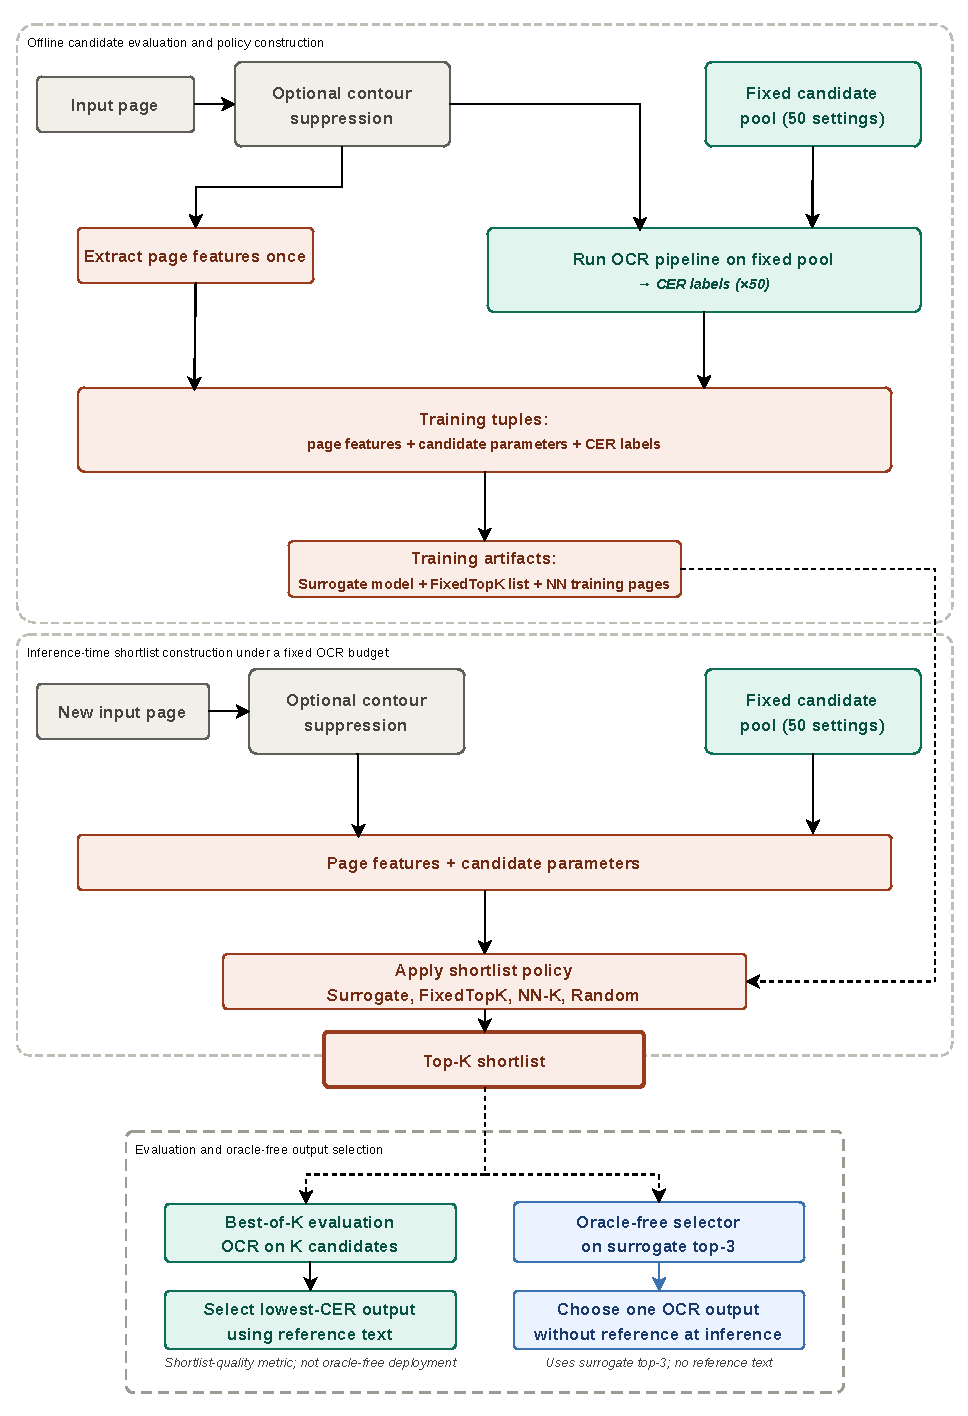
\includegraphics[width=0.90\textwidth,height=0.74\textheight,keepaspectratio]{pipeline_flowchart_2_5.pdf}
\caption{Proposed page-level preprocessing framework. In the offline stage, each page is optionally contour-suppressed, page features are extracted once, and a fixed pool of 50 preprocessing candidates is evaluated with OCR to obtain observed CER values for recognizer-specific surrogate training and baseline construction. At inference time, shortlist policies rank or transfer candidates for a new page under a limited OCR budget. The lower dashed branches distinguish best-of-K evaluation of shortlist quality from oracle-free selection of one output from the top-3 shortlist}
\label{fig:framework}
\end{figure*}

\subsection{Problem Formulation}

Let \(\mathcal{D}=\{(x_i,r_i)\}_{i=1}^{N}\) denote the page images and their reference transcriptions. The primary Vietnamese dataset has \(N=300\), and the SROIE receipt dataset has \(N=626\) after duplicate removal. Let \(\Theta=\{\theta_1,\ldots,\theta_M\}\) denote the fixed candidate pool of page-level preprocessing settings, with \(M=50\). For a given experimental setting, define the page representation as \(\tilde{x}_i=x_i\) in the raw setting and \(\tilde{x}_i=C(x_i)\) in the contour-suppressed setting, where \(C\) is the fixed contour-suppression transform described below.

For recognizer \(e\), the observed OCR response for page \(i\) and preprocessing candidate \(\theta_j\) is
\begin{equation}
y_{i,j,e}
=
\mathrm{CER}\left(O_e(P_{\theta_j}(\tilde{x}_i)), r_i\right),
\label{eq:ocr_response}
\end{equation}
where \(P_{\theta_j}\) applies the page-level preprocessing candidate and \(O_e\) denotes the OCR pipeline with the shared detector and recognizer \(e\). Page-level CER is computed from edit distance:
\begin{equation}
\mathrm{CER}(o,r)=\frac{S(o,r)+D(o,r)+I(o,r)}{|r|},
\label{eq:cer}
\end{equation}
where \(S\), \(D\), and \(I\) are the numbers of substitutions, deletions, and insertions needed to transform OCR output \(o\) into reference transcription \(r\).

For each page \(i\) and preprocessing candidate \(\theta_j\), the surrogate input is
\begin{equation}
z_{i,j} =
\left[f(\tilde{x}_i), \theta_j, g(f(\tilde{x}_i),\theta_j)\right]
\in \mathbb{R}^{22},
\label{eq:surrogate_input}
\end{equation}
where \(f(\tilde{x}_i)\) contains 12 OCR-free page features, \(\theta_j\) contains the 5 preprocessing parameters, and \(g(f(\tilde{x}_i),\theta_j)\) contains 5 predefined interaction terms between page properties and preprocessing controls, all defined in the remainder of Section~\ref{sec:method}; the 22-dimensional input thus comprises these three groups concatenated. A recognizer-specific surrogate \(h_e\) is trained as a supervised CER regressor that predicts \(\hat{y}_{i,j,e}=h_e(z_{i,j})\). Although trained as a CER regressor, the surrogate is used at inference time as a ranking function. The induced page-conditioned top-K shortlist policy is
\begin{equation}
\pi^{h_e}_K(\tilde{x}_i)
=
\operatorname*{Kmin}_{\theta_j\in\Theta} h_e(z_{i,j}),
\label{eq:topk_policy}
\end{equation}
where \(\operatorname*{Kmin}\) returns the \(K\) preprocessing candidates with the lowest predicted CER values.

The practical objective is therefore not exact CER prediction, but page-conditioned shortlist construction under a fixed OCR budget:
\begin{equation}
\begin{aligned}
\min_{\pi_K}
\mathbb{E}_{i}\left[
\min_{\theta_j \in \pi_K(\tilde{x}_i)} y_{i,j,e}
\right],
&\quad
\pi_K(\tilde{x}_i)\subset\Theta,\\
&\quad
|\pi_K(\tilde{x}_i)|=K.
\end{aligned}
\label{eq:selection_objective}
\end{equation}
This is an induced selection objective rather than the direct training loss. The surrogate is fitted to observed CER values, and its ranking is evaluated by the best observed CER within the selected top-K shortlist.

The reference baselines can be expressed in the same finite candidate pool. The sampled-pool oracle is
\begin{equation}
B^{\mathrm{oracle}}_{i,e}=\min_{\theta_j\in\Theta} y_{i,j,e},
\label{eq:sampled_oracle}
\end{equation}
which is the lowest observed CER within the sampled pool rather than a global optimum. The fixed baseline selects the single training-pool candidate with the lowest mean training CER, \(\theta^{*}_{\mathrm{fixed},e}=\arg\min_{\theta_j\in\Theta}\frac{1}{|\mathcal{I}_{\mathrm{train}}|}\sum_{i\in\mathcal{I}_{\mathrm{train}}} y_{i,j,e}\). Random K samples K candidates uniformly from the same \(\Theta\), while NoPre uses the exact OCR run with all preprocessing operations disabled.
We also define FixedTopK as a stronger static shortlist baseline: for each outer training fold, the K preprocessing candidates with the lowest mean training CER are selected and then applied as the same K-candidate shortlist to every held-out page.

\subsection{Contour Suppression as Upstream Page-Level Preprocessing}

As an optional preprocessing step, we use a fixed contour-based rule to identify rectangular regions that meet fixed criteria and replace their pixels with white before text detection. It is intended to reduce large non-text regions that can trigger false detections, such as stamps, decorative headers, logos, and watermarks, rather than to serve as a general artifact-removal method. Given an input page image, the method converts the image to grayscale, applies a Gaussian blur with a 5-by-5 kernel, computes an Otsu threshold, and extracts external contours from the inverted threshold mask. For each contour, a bounding rectangle is computed; if the rectangle satisfies all of the following criteria, it is overwritten with white pixels in the original image: contour area greater than 500 pixels, aspect ratio between 1.0 and 5.0, width greater than 80 pixels, and height greater than 30 pixels. A one-at-a-time robustness check on a 30-image subset found the aspect-ratio upper bound to be stable, while the area, minimum-width, and minimum-height thresholds affected CER more noticeably; we therefore treat contour suppression as a fixed, domain-motivated preprocessing condition rather than a fully optimized artifact-removal module. The output remains a page image rather than a binarized image; only selected large regions are suppressed. The objective is to reduce false detections before OCR, not to directly improve recognition in already detected text crops.

\subsection{Page-Level Preprocessing Search Space}

The page-level preprocessing search space has five tunable parameters applied to the grayscale page before text detection: \texttt{gaussian\_ksize} $\in \{0,3,5,7\}$, \texttt{bilateral\_d} $\in \{0,\ldots,9\}$, \texttt{clahe\_clip} $\in [0,4.0]$, \texttt{gamma} $\in [0.5,1.5]$, and \texttt{sharpen} $\in [0,2.0]$. These parameters correspond to Gaussian blur, bilateral filtering, CLAHE, gamma correction, and sharpening, respectively; their off/identity values and roles are tabulated in Online Resource 1.

These five controls were selected to address common page-level degradations using lightweight operations while keeping the search space compact and compatible with stratified sampling. Gaussian blur and bilateral filtering address noise under different smoothing assumptions, CLAHE targets local contrast and faded text, gamma correction adjusts global brightness, and sharpening addresses blurred strokes. We restrict the search to grayscale intensity operations that preserve page geometry and do not convert the image to a binary representation. Operations such as binarization and morphology would require categorical or pipeline-level design choices outside the fixed five-dimensional search space. Deskewing was not included because skew was minor across the 300 pages as measured by the \texttt{orig\_skew\_angle} feature in the current candidate data: no page exceeded $2^\circ$, and geometric correction is outside the intensity-based preprocessing scope studied here.

The two denoising parameters are discrete: \texttt{gaussian\_ksize=0} disables Gaussian blur, while positive values specify the Gaussian kernel size. Positive Gaussian kernel sizes are restricted to odd values, as required by the OpenCV implementation, and a kernel size of 1 is excluded because it is effectively an identity operation and redundant with the off value. Similarly, \texttt{bilateral\_d=0} disables bilateral filtering, while positive values specify the bilateral filter diameter. The remaining parameters are continuous, with \texttt{clahe\_clip=0} disabling CLAHE, \texttt{gamma=1.0} serving as the identity brightness transform, and \texttt{sharpen=0} disabling sharpening.

These ranges were retained after boundary checks that varied one parameter at a time on a subset of images across the three recognizers in both raw and contour-suppressed settings. The checks clearly supported the Gaussian upper bound; the other bounds were retained as common operating ranges rather than recognizer-specific optima.

Implementation settings outside this five-dimensional space are held fixed across all experiments: OpenCV automatic sigma for Gaussian blur, bilateral color and spatial sigma values of 75, an 8-by-8 CLAHE tile grid, and parametric 3-by-3 sharpening. Operations are applied in the fixed order Gaussian blur, bilateral filtering, CLAHE, gamma correction, and sharpening, with denoising before contrast/brightness adjustment and sharpening last to avoid amplifying earlier-stage noise.

\subsection{Data Collection via Stratified Candidate Sampling}

A fixed candidate pool of 50 preprocessing combinations is generated from a stratified five-dimensional unit-cube design, following the space-filling motivation of Latin hypercube sampling \cite{mckay1979lhs}, and then reused for every page. The two discrete parameters are obtained by binning the corresponding design coordinates into the discrete values actually used: \texttt{gaussian\_ksize} into \{0, 3, 5, 7\} and \texttt{bilateral\_d} into \{0, \ldots, 9\}. The three continuous parameters (\texttt{clahe\_clip}, \texttt{gamma}, and \texttt{sharpen}) are scaled linearly from their design coordinates into their stated ranges. This Latin-hypercube-style construction gives stratified one-dimensional coverage for the continuous parameters and near-balanced marginal counts for the discrete levels, while treating the 50 candidates as a compact finite design rather than a full factorial grid. For each page and candidate combination, the page is preprocessed, OCR is run, and page-level CER is computed against the reference transcription. This yields $300 \times 50 = 15{,}000$ rows per recognizer in the primary dataset, one for each page $i$ and candidate $\theta_j$, with each row storing page features, preprocessing parameters, and the observed CER after OCR.

The candidate-pool design aims for broad coverage of the preprocessing response surface rather than per-image convergence to an optimum; with $D=5$ search dimensions, $M=50$ follows the common $n\approx 10d$ rule of thumb for initial space-filling computer experiments \cite{loeppky2009sample}. The sampled-pool oracle reported in the experiments therefore refers to the best observed configuration within this finite pool, not a global optimum over the continuous preprocessing space. The offline OCR evaluation loop is summarized in Online Resource 1.

\subsection{Page-Level Features}

For each page, image features that do not require OCR are extracted once before evaluating candidate preprocessing settings. In the raw setting, features are computed from the original page image; in the contour-suppressed setting, they are computed from the contour-suppressed page image. The base feature set contains seven intensity and texture descriptors: blur, contrast, brightness, noise, edge density, entropy, and dynamic range. We also include five document-aware descriptors: text density, skew angle, connected-component count, aspect ratio, and estimated line count. The base features capture low-level image quality, tone, and texture, whereas the document-aware descriptors capture page structure that is not represented by intensity statistics alone.

The surrogate input concatenates these 12 page-level features with the five preprocessing parameters. In addition, we include five predefined interaction terms that pair each preprocessing control with the image property it is intended to address: blur $\times$ \texttt{gaussian\_ksize}, contrast $\times$ \texttt{clahe\_clip}, brightness $\times$ \texttt{gamma}, noise $\times$ \texttt{bilateral\_d}, and entropy $\times$ \texttt{sharpen}. These interactions encode predefined, domain-motivated assumptions about how the effect of each preprocessing operation depends on page properties, without performing data-driven feature selection over a larger interaction pool. The resulting surrogate input has 22 dimensions: 12 page features, 5 preprocessing parameters, and 5 interaction terms.

We use OCR-free hand-crafted page features rather than learned visual embeddings to keep the ranking model lightweight and independent of any additional pretrained image model at inference time. The feature definitions also allow domain-motivated interaction terms that directly pair image properties with the preprocessing controls they are intended to modulate. The effect of these feature groups is evaluated empirically in the ablation study in Section~\ref{sec:results}; the full feature-group table is provided in Online Resource 1.

\subsection{Surrogate Model}

For each recognizer, we train a separate surrogate regressor to predict page-level CER for a given page and preprocessing candidate. The input is the 22-dimensional vector described above, and the target is the actual CER obtained after applying the candidate preprocessing setting and running the OCR pipeline. The surrogate is therefore recognizer-specific but shares the same feature representation and candidate pool across recognizers.

The surrogate is used for ranking rather than for exact CER prediction. For each held-out page, the model scores every candidate preprocessing combination in the fixed candidate pool, and candidates with lower predicted CER are ranked higher. We refer to this as a cross-instance surrogate because the model is trained across many pages and reused for unseen pages, rather than being fitted separately for each page through iterative feedback.

We use regression followed by ranking rather than a direct pairwise or listwise learning-to-rank objective for two practical reasons. First, the observed target is a continuous page-level CER, and calibrated CER predictions are useful beyond candidate ordering: they define Top1Pred, prediction margins, and features for the oracle-free top-3 selector. Second, the main methodological question is whether page-conditioned scoring can enrich a small shortlist under a fixed OCR-call budget, not which tabular ranking loss is optimal. Direct learning-to-rank models are therefore left as an extension rather than treated as a primary contribution.

We consider four regression model families: Ridge regression, Random Forest, XGBoost, and LightGBM. These families cover linear, bagged-tree, and gradient-boosted regressors commonly used for feature-based tabular regression. Model-family selection and evaluation are performed within the nested GroupKFold protocol described in Section~\ref{sec:experimental_setup}. We do not include stacking in the primary evaluation because group-aware out-of-fold predictions would be needed to train a stacking meta-learner without mixing candidate rows from the same page.

\subsection{Evaluation Protocol}

We evaluate shortlist quality under fixed OCR-call budgets $K \in \{3, 5, 10, 15\}$. These values span tight to moderate budgets, covering 6\% to 30\% of the 50-candidate pool. For each held-out page, the surrogate ranks the fixed 50-candidate pool by predicted CER, and the Surrogate K shortlist consists of the K candidates with lowest predicted CER. The Random K baseline samples K candidates uniformly from the same pool; to reduce Monte Carlo noise, random results are averaged over 20 reproducible trials per page without requiring additional OCR runs, since all trials resample from the already evaluated candidate pool. FixedTopK selects the K candidates with the lowest mean training CER in each outer fold and uses that same static shortlist for every held-out page. Surrogate K, Random K, and FixedTopK are evaluated using best-of-K CER, defined as the minimum actual CER among the K candidates in the shortlist.

As an additional retrieval-based baseline, we evaluate a nearest-neighbor transfer shortlist (NN-K) in the Vietnamese raw, contour-suppressed, and SROIE settings. For each outer fold, page features are standardized using only the training pages. For each held-out page, NN-K finds the nearest training pages in this OCR-free feature space, transfers the oracle-best preprocessing candidate from each nearest training page, removes duplicate candidates while preserving neighbor order, and fills any remaining shortlist slots with fold-specific FixedTopK candidates if needed. NN-K therefore uses only training-fold OCR responses for candidate transfer and is evaluated on held-out pages with the same best-of-K protocol as Surrogate K and FixedTopK.

We also report three reference baselines. No preprocessing uses exact OCR runs with all preprocessing operations disabled. FixedBest selects, within each training fold, the single preprocessing combination with the lowest mean CER on the training pages and applies it to the held-out pages. Sampled Oracle is the minimum actual CER among all 50 sampled candidates for each page; it is the lowest observed CER within the sampled candidate pool, not the true global optimum over all preprocessing parameters.

We report computational cost primarily in OCR-call units because OCR runtime depends on hardware, recognizer implementation, and page content. The offline data collection stage requires 50 OCR evaluations per page and is used only to build the training and evaluation table. At inference time, OCR-free feature extraction and scoring the 50 tabular candidate rows require no additional OCR calls, but their wall-clock overhead is not benchmarked here. NoPre, FixedBest, and Top1Pred require one OCR call per page; the oracle-free top-3 selector requires three OCR calls; Surrogate K, NN-K, and FixedTopK require K OCR calls under the best-of-K shortlist-quality protocol; and the sampled-pool oracle requires all 50 OCR calls. OCR-call count therefore captures the repeated inference budget, while hardware-specific end-to-end latency remains outside the scope of this study.

Because Surrogate K and Random K both use best-of-K selection during evaluation, these results measure shortlist quality under a fixed candidate-evaluation budget rather than oracle-free output-selection performance. The comparison remains fair because both methods receive the same within-shortlist best-of-K evaluation. We additionally compute an oracle-free one-call operating point, Top1Pred, defined as the single candidate with the lowest out-of-fold predicted CER. Top1Pred does not use reference text or within-shortlist CER selection; it is reported as a supplementary single-output baseline rather than as the main shortlist-quality metric.

To test whether a short surrogate shortlist can be used without reference text at inference time, we also evaluate an oracle-free top-3 output selector. For each held-out page, OCR is run on the surrogate-ranked top-3 candidates and the selector chooses one of the three OCR outputs. Candidate-level selector features include the surrogate rank, predicted CER and prediction margins, preprocessing parameters, the number of detected crops, OCR text length and character-composition statistics, simple document-pattern counts such as dates and administrative keywords, and agreement features based on normalized edit distances among the three OCR outputs. We compare five selector families: random-forest and logistic-regression classifiers trained to identify the best candidate within the top-3, and random-forest, gradient-boosting, and ridge regressors trained to predict candidate CER. Selector-family choice is nested inside each outer fold: the family with the lowest inner-fold validation CER on the outer-training pages is refit on all outer-training pages and then used on the held-out pages. The held-out selector therefore uses OCR outputs, surrogate predictions, and preprocessing metadata, but not reference text or held-out CER values. We compare it with Top1Pred, the agreement-only baseline, FixedBest, NoPre, and the best-of-3 oracle. The agreement-only baseline selects the top-3 output with the smallest mean normalized edit distance to the other two outputs.

For a feature-matched sensitivity analysis, we replace the surrogate's predicted CER and prediction-margin features by the within-shortlist ranks 1, 2, and 3. The exact surrogate top-3 candidates, OCR outputs, and all remaining selector features are retained, and the nested selector is rerun. This makes the prediction-related inputs comparable with NN-K and FixedTopK, which provide an ordering but not a continuous CER prediction. The analysis tests whether policy comparisons persist without the surrogate's numerical score and margin information. It is not a pure test of shortlist quality because the selector is refit and continues to use OCR-output features.

\section{Experimental Setup}
\label{sec:experimental_setup}

\subsection{OCR Recognizers}

All primary experiments use the same text-detection stage: PaddleOCR detection with Vietnamese configuration (\texttt{lang=vi}). The detected text regions are cropped and passed to one of three recognizers: VietOCR, Tesseract with the Vietnamese language pack (\texttt{vie}), and EasyOCR with Vietnamese recognition (\texttt{vi}). Thus, the detector and page-level preprocessing pipeline are held fixed while the recognizer changes.

The final candidate-response data were generated with PaddleOCR~3.3.2 on PaddlePaddle GPU~3.3.0, VietOCR~0.3.13 using its \texttt{vgg\_transformer} configuration, EasyOCR~1.7.2, and Tesseract~5.3.4 through \texttt{pytesseract}~0.3.13. The installed Tesseract \texttt{eng} and \texttt{vie} language packages were version \texttt{1:4.1.0-2}. For each page, detector polygons were converted to axis-aligned bounding-rectangle crops and processed in the \texttt{dt\_polys} order returned by PaddleOCR; no additional reading-order sorting was applied. Nonempty recognized strings were joined with tab separators in that preserved order. VietOCR output was retained only when its predicted confidence was strictly greater than 0.8. Tesseract was called with its default engine and page-segmentation settings.

PaddleOCR was used as the shared detector because it supports a modular pipeline in which one detector can be paired with multiple recognizers. Keeping detection fixed lets the experiments focus on preprocessing selection rather than detector choice. The recognizers were chosen to cover complementary practical OCR backends: VietOCR as a Vietnamese-specific neural recognizer, Tesseract as a mature open-source OCR engine with LSTM recognition, and EasyOCR as a general-purpose neural OCR toolkit. These backends are used here to test whether preprocessing-selection behavior changes across recognizers, not as the main optimization target. For the SROIE setting described in Section~\ref{sec:dataset_problem}, the same detector-recognizer structure is used with English configurations, and VietOCR is omitted because it is Vietnamese-specific.

\subsection{Nested GroupKFold Cross-Validation}

For the Vietnamese experiments, all reported surrogate results are computed with a nested 5-fold GroupKFold protocol, using the page image as the grouping unit. All 50 candidate preprocessing rows from the same page are kept in the same fold, preventing leakage in which candidates from one page appear in both training and test data. Each outer fold therefore evaluates the selected surrogate on held-out pages that were not used to fit that fold's model. After the five outer folds are completed, the held-out page-level results are combined across folds, giving one out-of-fold result for each of the 300 pages. The same group-aware nested protocol is used for the SROIE setting, with results combined over all 626 receipt images.

Model-family selection is nested inside each outer training fold. For each recognizer and outer fold, the candidate model families are compared using inner GroupKFold on the outer-training pages, and the family with the lowest mean validation MAE is selected. That selected family is then refit on the full outer-training fold and evaluated on the corresponding held-out fold. This nested protocol avoids selecting a model family using information from the outer test pages, following standard guidance on reducing selection-induced optimism in cross-validation \cite{varma2006bias,cawley2010overfitting,parvandeh2020consensus}.

A final model is also selected and refit on all available pages for saved inference artifacts, but this final model is not used to compute the reported cross-validation metrics. A compact protocol table and stepwise nested-evaluation algorithm are provided in Online Resource 1.

\subsection{Metrics}

CER is the primary OCR-quality metric and is computed at the page level against the reference transcription. Surrogate prediction quality is summarized using MAE and $R^2$. We report two Spearman rank correlations: global Spearman, computed over all held-out candidate rows within an outer fold, and per-image Spearman, computed as the mean within-page candidate-rank correlation over held-out pages. Per-image Spearman is most directly aligned with the shortlist objective because the surrogate must rank the fixed candidate pool separately for each test page. Best-of-K CER evaluates the actual CER achieved by the best observed candidate within the surrogate-ranked shortlist.

For statistical comparison, Surrogate K is compared with Random K and FixedTopK using two-sided paired Wilcoxon signed-rank tests over page-level best-of-K CER values. The supplementary NN-K baseline is compared with Surrogate K, FixedTopK, and Random K using the same two-sided paired page-level tests. The oracle-free top-3 selector is compared with Top1Pred, the agreement-only baseline, and FixedBest using two-sided paired page-level tests. Tests are run separately for each recognizer, setting, and K value where applicable, and the direction of an effect is reported from the paired mean CER difference. Aggregate CER values are reported as means over the held-out page-level results combined across outer folds. We also compute percentile bootstrap confidence intervals for paired mean differences, with Surrogate K minus the corresponding baseline as the signed difference. Random K is estimated as the mean best-of-K CER over 20 reproducible random draws per page.

For the retrospective headroom analysis, let \(F_{i,K}\) be the fold-specific FixedTopK CER, \(O_i\) the sampled-pool-oracle CER, and \(P_{i,K}\) the CER of policy \(P\). We define headroom \(H_{i,K}=F_{i,K}-O_i\) and FixedTopK-relative policy advantage \(A_{i,K}^{P}=F_{i,K}-P_{i,K}\). These quantities share \(F_{i,K}\), and \(A_{i,K}^{P}\leq H_{i,K}\) because the sampled-pool oracle is the best candidate in the pool. We therefore compute the coupled correlation for Surrogate, Random, and NN-K, and separately correlate headroom with direct policy-to-policy gains that do not contain FixedTopK: Random minus Surrogate, Random minus NN-K, and NN-K minus Surrogate. This control analysis is descriptive and is not used for model or policy selection.

Because the study reports multiple paired comparisons, p-values are interpreted within predefined comparison families rather than as a single global null-hypothesis test. For the eight selector-versus-FixedBest comparisons, we report both unadjusted p-values and Holm-adjusted significance across the family. We emphasize repeated directionally consistent patterns, paired mean differences, and bootstrap confidence intervals, and we avoid drawing strong conclusions from isolated marginal tests. Accordingly, the conclusions emphasize the repeated surrogate-versus-random results, the SROIE surrogate-versus-FixedTopK pattern, and the setting-dependent surrogate-versus-NN-K comparisons.

\subsection{Hyperparameters and Sensitivity}

The primary results use the nested GroupKFold protocol described above, with model-family selection performed inside each outer training fold. For implementation-level regressor settings, we do not run a broad hyperparameter search. Instead, we compare four predefined surrogate model families, chosen to cover common linear, bagged-tree, and gradient-boosted regressors, with fixed hyperparameters for each family. The goal is not to exhaustively benchmark surrogate regressors, but to evaluate whether a practical cross-instance surrogate can provide useful shortlist rankings. This keeps the focus on candidate ranking under a fixed OCR budget rather than on maximizing a standalone regressor benchmark.

As a sensitivity check, we also reran the surrogate evaluation with default regressor settings in supplementary holdout experiments for both raw and contour-suppressed images. These reruns preserved the main significance pattern: surrogate shortlists remained significantly better than random shortlists in all 12/12 raw comparisons and all 12/12 contour comparisons. We therefore treat the nested GroupKFold results as the primary evidence and the default-parameter reruns as supplementary evidence that the surrogate-vs-random conclusion is not fragile to the chosen regressor settings.

\subsection{Use of AI Tools}

Large language models---Claude (Anthropic) and Codex (OpenAI)---assisted with drafting some analysis and evaluation scripts. The authors verified all reported results, numerical values, and scientific claims and take full responsibility for the manuscript.

\section{Results}
\label{sec:results}

\subsection{Preprocessing Response Variation in the Fixed Candidate Pool}

PaddleOCR detection settings are held fixed throughout the main multi-recognizer experiments. This isolates the page-level preprocessing-selection problem and keeps the detector shared across the three recognizers. We next quantify the observed preprocessing-response variation within the fixed candidate pool.

The 50-candidate pool exhibits substantial within-page variation. Mean within-image CER coefficients of variation are 55.5\%, 67.1\%, and 25.1\% for raw VietOCR, Tesseract, and EasyOCR, and 68.9\%, 77.5\%, and 29.4\% after contour suppression. The sampled-pool oracle improves over exact NoPre on 90--98\% of pages, with mean relative CER reductions of 15.3--38.2\% across the six settings (full results in Online Resource 1). Because this oracle evaluates all 50 candidates, it is not deployable; it establishes that the pool contains useful choices that a budgeted policy should retrieve.

\subsection{Surrogate Model Quality}

The surrogate models show moderate CER prediction accuracy and rank correlation. Across the six Vietnamese recognizer-setting combinations, nested-CV $R^2$ ranges from 0.435 to 0.614, global Spearman from 0.522 to 0.676, and mean per-image Spearman from 0.497 to 0.776; full fold-level model-quality metrics are given in Online Resource 1. Per-image Spearman is most directly aligned with the shortlist objective because each test page requires ranking the same 50 preprocessing candidates for that page. Because absolute prediction metrics and global rank correlation do not by themselves determine shortlist quality, we next evaluate it directly using best-of-K CER.

\subsection{Surrogate Shortlists vs Random Shortlists}

Under the same K-candidate budget, two-sided paired Wilcoxon tests show lower CER for surrogate shortlists than for random shortlists across all three recognizers, all evaluated K values, and both raw and contour-suppressed settings. The raw setting has 12/12 significant surrogate-vs-random comparisons, the contour-suppressed setting also has 12/12, giving 24/24 significant comparisons overall. Best-of-K curves across recognizers and budgets are visualized in Online Resource 1.

The effect-size pattern is consistent with the budgeted-ranking interpretation: surrogate gains over random are largest at small K and generally decrease as K grows, because random shortlists become more likely to contain a good candidate when the shortlist budget increases. The gains are largest for EasyOCR and smallest for VietOCR, which has the lowest NoPre CER in the Vietnamese experiments. The stronger FixedTopK baseline is more competitive than Random K, however, and is analyzed separately below.

\begin{table*}[t]
\centering
\caption{Vietnamese best-of-K CER results. Values are percentages. Each S/R entry reports Surrogate K / Random K.}
\label{tab:vn_bestk}
\small
\resizebox{\textwidth}{!}{%
\begin{tabular}{l l r r r c c c c}
\toprule
Setting & Recognizer & NoPre & FixedBest & SampOracle & K=3 S/R & K=5 S/R & K=10 S/R & K=15 S/R \\
\midrule
Raw & VietOCR & 4.70 & 4.63 & 3.61 & 4.23 / 4.53 & 4.10 / 4.25 & 3.87 / 3.98 & 3.79 / 3.86 \\
Raw & Tesseract & 9.82 & 9.29 & 6.85 & 8.29 / 8.98 & 7.86 / 8.40 & 7.46 / 7.77 & 7.20 / 7.50 \\
Raw & EasyOCR & 15.44 & 15.19 & 13.19 & 14.27 / 15.75 & 13.94 / 15.18 & 13.57 / 14.41 & 13.42 / 14.07 \\
Contour & VietOCR & 3.15 & 3.19 & 2.31 & 2.89 / 3.08 & 2.77 / 2.84 & 2.58 / 2.61 & 2.50 / 2.51 \\
Contour & Tesseract & 7.69 & 7.28 & 5.19 & 6.49 / 6.98 & 6.15 / 6.50 & 5.70 / 5.94 & 5.49 / 5.71 \\
Contour & EasyOCR & 13.25 & 13.09 & 11.10 & 12.35 / 13.64 & 11.97 / 13.06 & 11.58 / 12.31 & 11.37 / 11.97 \\
\bottomrule
\end{tabular}%
}
\end{table*}

\subsection{Comparison with FixedTopK Static Shortlists}

Table~\ref{tab:fixedtopk_comparison} summarizes the comparison with FixedTopK at the tightest and largest evaluated shortlist budgets. FixedTopK is a strong static baseline and is generally much stronger than random selection, although it is nearly tied with random in the lowest-error contour-suppressed VietOCR cases at larger K. Two-sided paired Wilcoxon tests show significant surrogate improvements over FixedTopK at $p<0.05$ in 5/12 raw Vietnamese comparisons and 8/8 SROIE comparisons. In the contour-suppressed Vietnamese setting, no comparison significantly favors the surrogate, while 2/12 comparisons significantly favor FixedTopK. Bootstrap intervals for the paired mean difference (Surrogate minus FixedTopK) give a compatible interpretation. In the raw Vietnamese setting, four of 12 intervals favor the surrogate, one favors FixedTopK, and seven overlap zero. In the contour-suppressed setting, no interval favors the surrogate, three favor FixedTopK, and nine overlap zero. On SROIE, all eight intervals favor the surrogate. In mean CER, Tesseract favors FixedTopK at $K=3$ in both raw and contour-suppressed Vietnamese settings, with differences of +0.19 percentage points and +0.33 percentage points, respectively; the latter has a 95\% interval of [+0.16, +0.55]. On SROIE, by contrast, all intervals are negative, for example -1.04 percentage points for Tesseract at $K=3$ with a 95\% interval of [-1.33, -0.76]. These results show that the added value of page-conditioned ranking over a strong static shortlist is dataset- and recognizer-dependent.

\begin{table*}[t]
\centering
\caption{Comparison with FixedTopK static shortlists. CER values are percentages. Diff is Surrogate minus FixedTopK, so negative values favor the surrogate.}
\label{tab:fixedtopk_comparison}
\small
\resizebox{\textwidth}{!}{%
\begin{tabular}{l l r r r r r r}
\toprule
Setting & Recognizer & Surr K=3 & FixedTopK K=3 & Diff K=3 & Surr K=15 & FixedTopK K=15 & Diff K=15 \\
\midrule
Raw & VietOCR & 4.23 & 4.27 & -0.04 & 3.79 & 3.85 & -0.07 \\
Raw & Tesseract & 8.29 & 8.11 & 0.19 & 7.20 & 7.30 & -0.10 \\
Raw & EasyOCR & 14.27 & 14.33 & -0.05 & 13.42 & 13.50 & -0.08 \\
Contour & VietOCR & 2.89 & 2.87 & 0.02 & 2.50 & 2.51 & -0.02 \\
Contour & Tesseract & 6.49 & 6.16 & 0.33 & 5.49 & 5.46 & 0.03 \\
Contour & EasyOCR & 12.35 & 12.22 & 0.13 & 11.37 & 11.37 & 0.00 \\
SROIE & Tesseract & 43.23 & 44.27 & -1.04 & 40.99 & 41.44 & -0.44 \\
SROIE & EasyOCR & 39.08 & 39.22 & -0.14 & 38.17 & 38.28 & -0.11 \\
\bottomrule
\end{tabular}%
}
\end{table*}

\subsection{Policy-Agnostic FixedTopK-to-Oracle Headroom}
\label{sec:gap_diagnostic}

The aggregate comparison above shows that FixedTopK leaves different amounts of residual improvement across pages and settings. We quantify this as the per-page headroom \(H_{i,K}=F_{i,K}-O_i\). A surrogate-only analysis would compare it with \(F_{i,K}-S_{i,K}\), the surrogate's advantage over FixedTopK. However, the two quantities share \(F_{i,K}\), and the sampled-pool oracle enforces \(F_{i,K}-P_{i,K}\leq H_{i,K}\) for every pool-constrained policy \(P\). A positive correlation can therefore reflect this construction rather than a learned-ranking effect.

We assess the relationship using the same held-out pages for Surrogate, Random, and NN-K. As Table~\ref{tab:headroom_controls} shows, each coupled FixedTopK-relative advantage has a significantly positive correlation with headroom in all 32 combinations of recognizer, setting, and budget, and the highest-headroom quartile has a larger mean advantage than the lowest quartile in all 32 configurations for every policy. Random's correlation is larger than the surrogate's in 30/32 configurations. Thus, the original 32/32 pattern is policy-agnostic and cannot establish that high-headroom pages specifically favor learned ranking.

We additionally correlate headroom with direct policy-to-policy gains that do not contain FixedTopK. The correlation between headroom and Random minus Surrogate ranges from $-0.516$ to $0.022$, with no significantly positive result; headroom versus NN-K minus Surrogate is negative in all 32 configurations. The NN-K-versus-Random control is mixed, with significantly positive correlations in 5/32 configurations. These controls do not support using headroom alone to select among Surrogate, NN-K, and Random.

\begin{table*}[t]
\centering
\caption{Policy-agnostic headroom controls over 32 dataset/setting/recognizer/budget configurations. Coupled outcomes share FixedTopK with headroom; non-shared outcomes are direct policy-to-policy gains. Positive sig. counts significantly positive Spearman correlations ($p<0.05$); Q4$>$Q1 counts configurations whose highest-headroom quartile has a larger mean outcome than the lowest.}
\label{tab:headroom_controls}
\small
\resizebox{\textwidth}{!}{%
\begin{tabular}{l l r r r}
\toprule
Analysis & Outcome & Spearman $r$ range & Positive sig. & Q4$>$Q1 \\
\midrule
Coupled & FixedTopK $-$ Surrogate & [0.324, 0.638] & 32/32 & 32/32 \\
Coupled & FixedTopK $-$ Random & [0.359, 0.843] & 32/32 & 32/32 \\
Coupled & FixedTopK $-$ NN-K & [0.395, 0.759] & 32/32 & 32/32 \\
\midrule
Non-shared & Random $-$ Surrogate & [$-0.516$, 0.022] & 0/32 & 1/32 \\
Non-shared & Random $-$ NN-K & [$-0.286$, 0.191] & 5/32 & 11/32 \\
Non-shared & NN-K $-$ Surrogate & [$-0.370$, $-0.066$] & 0/32 & 0/32 \\
\bottomrule
\end{tabular}%
}
\end{table*}

\begin{figure*}[t]
\centering
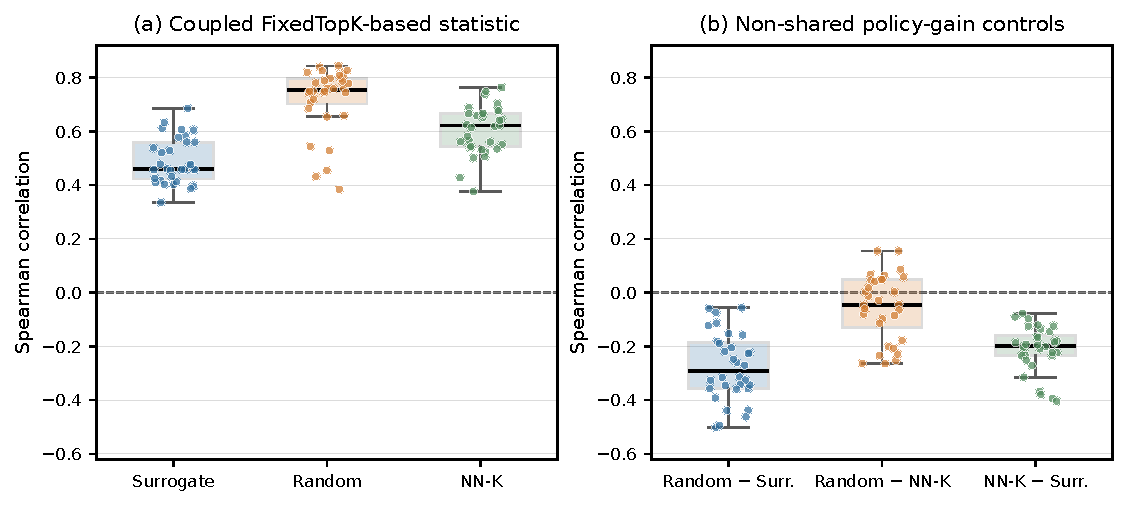
\includegraphics[width=0.88\textwidth]{headroom_policy_controls.pdf}
\caption{Spearman correlations across all 32 dataset/setting/recognizer/budget configurations. Each point is one configuration and the dashed line marks zero. (a) Headroom versus FixedTopK-relative advantage is positive for Surrogate, Random, and NN-K, consistent with the shared FixedTopK term and oracle constraint. (b) Direct policy-to-policy gains remove the shared term and show no corresponding positive pattern for learned ranking. Boxes show the median and interquartile range}
\label{fig:gap_diagnostic}
\end{figure*}

Headroom remains a valid retrospective description of how far FixedTopK lies from the best candidate observed in the finite pool. It requires labeled historical data and evaluation of the pool, and it does not identify which alternative policy will achieve that improvement. Evidence about policy quality therefore comes from the direct mean-CER, paired-test, and oracle-free selector comparisons reported in the surrounding sections.

\subsection{Nearest-Neighbor Transfer Baseline}

NN-K outperforms Random K in every evaluated comparison, confirming useful transfer from OCR-free page features. Neither page-conditioned policy dominates: the surrogate is stronger for raw EasyOCR and SROIE Tesseract mainly at small budgets, while NN-K is competitive or better for VietOCR and small-budget SROIE EasyOCR. Vietnamese differences are generally small, especially after contour suppression; full paired comparisons are provided in Online Resource 1 and the public result tables.

\subsection{VietOCR in the Lowest-Baseline-CER Setting}

Despite its low baseline CER, VietOCR benefits at $K=3$: raw CER is 4.23\% for Surrogate versus 4.70\% NoPre, 4.63\% FixedBest, and 4.53\% Random; contour CER is 2.89\% versus 3.15\%, 3.19\%, and 3.08\%, respectively.

\subsection{Contour Suppression as a Complementary Stage}

Contour suppression removes large rectangular non-text regions before detection, whereas the surrogate ranks photometric settings. It lowers NoPre CER from 4.70\% to 3.15\% (VietOCR), 9.82\% to 7.69\% (Tesseract), and 15.44\% to 13.25\% (EasyOCR); contour + Surrogate $K=15$ reaches 2.50\%, 5.49\%, and 11.37\%, respectively. Online Resource 1 illustrates the operation.

\subsection{Feature Ablation}

Document-aware features matter most for Tesseract: removing them lowers global Spearman/$R^2$ from 0.674/0.614 to 0.512/0.229 raw and from 0.586/0.576 to 0.508/0.369 contour; EasyOCR degrades more moderately and VietOCR changes are mixed. Removing interactions changes global Spearman by about $\pm0.015$ and $K=3$ CER by at most 0.13 points. All 12 surrogate-vs-random comparisons remain significant under every ablation, so these changes affect surrogate metrics more than the main shortlist conclusion.

\subsection{SROIE Evaluation: Surrogate Outperforms FixedTopK}

The SROIE evaluation applies the same full-page shortlist-ranking protocol to a different document domain and English OCR configuration. Unlike the Vietnamese settings, the surrogate directly outperforms FixedTopK across all evaluated SROIE recognizer-budget comparisons. SROIE also has greater aggregate FixedTopK-to-oracle headroom, but Section~\ref{sec:gap_diagnostic} shows that headroom alone does not explain which policy will perform best.

\begin{table*}[t]
\centering
\caption{SROIE receipt-setting results. CER values are percentages.}
\label{tab:sroie_results}
\small
\resizebox{\textwidth}{!}{%
\begin{tabular}{l r r r r r r r r r r r r r r}
\toprule
Recognizer & $R^2$ & Global Spearman & Per-image Spearman & NoPre & FixedBest & SampOracle & Surr K=3 & NN K=3 & FixedTopK K=3 & Rand K=3 & Surr K=15 & NN K=15 & FixedTopK K=15 & Rand K=15 \\
\midrule
Tesseract & 0.480 & 0.674 & 0.588 & 50.52 & 46.80 & 40.17 & 43.23 & 43.68 & 44.27 & 46.54 & 40.99 & 41.03 & 41.44 & 42.22 \\
EasyOCR & 0.609 & 0.672 & 0.664 & 40.85 & 40.06 & 37.88 & 39.08 & 38.81 & 39.22 & 40.81 & 38.17 & 38.14 & 38.28 & 38.59 \\
\bottomrule
\end{tabular}%
}
\end{table*}

The omitted $K=5,10$ rows follow the same pattern and appear in Online Resource 1. All eight surrogate-vs-random and surrogate-vs-FixedTopK tests favor the surrogate; NN-K also beats FixedTopK and Random, but its ordering against the surrogate depends on recognizer and budget. These full-page, strict-CER results are not receipt key-information-extraction or cropped-field benchmarks.

\subsection{Oracle-Free Top-3 Output Selection}

Best-of-K uses observed within-shortlist CER. As an oracle-free check, Table~\ref{tab:oracle_free_selector} reports the nested selector using only the surrogate top-3 OCR outputs and derived prediction, text-quality, and agreement features. Its comparisons with Top1Pred, agreement-only, FixedBest, and NoPre are one-output CERs.

\begin{table*}[t]
\centering
\caption{Oracle-free top-3 output-selection results. CER values are percentages. Sel-Fixed is Selector minus FixedBest, so negative values favor the selector. Reported p-values are two-sided paired Wilcoxon tests for Selector versus FixedBest.}
\label{tab:oracle_free_selector}
\small
\resizebox{\textwidth}{!}{%
\begin{tabular}{l l r r r r r r r}
\toprule
Setting & Recognizer & Selector & Top1Pred & Agreement & FixedBest & NoPre & Sel-Fixed & $p$(Selector vs FixedBest) \\
\midrule
Raw & VietOCR & 4.52 & 4.66 & 4.60 & 4.63 & 4.70 & -0.11 & $9.18{\times}10^{-5}$ \\
Raw & Tesseract & 8.97 & 9.47 & 9.11 & 9.29 & 9.82 & -0.32 & 0.0126 \\
Raw & EasyOCR & 14.98 & 15.19 & 15.27 & 15.19 & 15.44 & -0.22 & 0.112 \\
Contour & VietOCR & 3.19 & 3.20 & 3.16 & 3.19 & 3.15 & -0.00 & 0.142 \\
Contour & Tesseract & 7.04 & 7.58 & 7.12 & 7.28 & 7.69 & -0.23 & 0.0151 \\
Contour & EasyOCR & 12.92 & 13.01 & 13.07 & 13.09 & 13.25 & -0.17 & 0.0313 \\
SROIE & Tesseract & 44.29 & 46.21 & 45.68 & 46.80 & 50.52 & -2.51 & $4.63{\times}10^{-37}$ \\
SROIE & EasyOCR & 39.80 & 40.13 & 40.03 & 40.06 & 40.85 & -0.26 & 0.000563 \\
\bottomrule
\end{tabular}%
}
\end{table*}

The selector has lower mean CER than Top1Pred in all eight rows; six paired comparisons remain significant after Holm correction across this eight-comparison family, with contour VietOCR and contour EasyOCR as the exceptions. Against FixedBest, the selector has lower mean CER in all eight settings. Six paired tests have unadjusted $p<0.05$; after Holm correction across the eight selector-versus-FixedBest comparisons, raw VietOCR and both SROIE recognizers remain significant. The largest reduction is SROIE Tesseract: 44.29\% versus 46.80\% FixedBest and 46.21\% Top1Pred. Thus, top-3 output selection recovers part, but not all, of the best-of-3 oracle gain.

\subsection{Feature-Matched Selector Sensitivity Analysis}

Replacing continuous surrogate predictions and margins with ranks preserves the exact top-3 candidates while matching the information available to NN-K and FixedTopK. After Holm correction over 14 comparisons, this selector beats NN-K for raw VietOCR ($-0.21$ points), raw EasyOCR ($-0.34$), and contour EasyOCR ($-0.43$); the other Vietnamese comparisons are nonsignificant. No Vietnamese FixedTopK comparison is significant. On SROIE, it beats FixedTopK for Tesseract by $-0.86$ points (95\% CI [$-1.20,-0.52$]) but not EasyOCR. Full results and the reason for omitting the SROIE NN-K comparison are documented in Online Resource 1.

\section{Discussion}
\label{sec:discussion}

\subsection{Ranking Utility Despite Moderate R-squared}

Moderate $R^2$ does not preclude useful shortlists because the objective is to place strong candidates near the top, not to estimate every CER exactly. The nested per-image rank correlations and consistently better-than-random shortlists show that within-page ordering can suffice.

\subsection{Interpreting Policy Comparisons and Available Headroom}

FixedTopK transfers well on the more homogeneous Vietnamese pages, particularly after contour suppression, whereas the surrogate consistently improves over it on SROIE; NN-K is also competitive. This setting-dependent pattern precludes a universal policy ranking. Contour VietOCR at $K=10,15$ further shows that statistically directional differences can be practically negligible (at most about 0.03 CER points).

FixedTopK-to-oracle headroom indicates residual improvement in the sampled pool, but its correlation with every FixedTopK-relative advantage, including Random, follows from the shared term and oracle constraint. It therefore requires labeled full-pool data and cannot choose a policy; direct held-out comparisons remain necessary.

\subsection{Surrogate Ranking and Retrieval-Based Transfer}

NN-K transfers candidates from similar pages rather than learning a CER function over $(i,\theta_j)$. Its advantage over Random confirms informative page features, while its mixed comparison with the surrogate suggests complementary empirical behavior rather than causal superiority of either method.

At the best-of-K level, Surrogate versus NN-K remains setting-dependent. At the output-selection level, feature matching retains three significant Vietnamese advantages over NN-K and the SROIE Tesseract advantage over FixedTopK. Because the selector is refit and retains OCR-output features, this is a targeted robustness check, not a pure shortlist comparison or evidence of universal superiority.

\subsection{Practical Interpretation of K}

$K$ is a shortlist-quality budget: the four policies report the best observed CER within a $K$-candidate shortlist, not a deployable one-output choice. Top1Pred is a one-call operating point, whereas the nested selector produces one output from three OCR calls.

\section{Limitations}
\label{sec:limitations}

\begin{enumerate}
    \item Best-of-K measures shortlist quality, not oracle-free deployment. The supervised top-3 selector uses three OCR calls and OCR-output features; feature matching removes its numerical score advantage but is still not a pure shortlist test.
    \item No non-random policy wins universally: FixedTopK is strong on Vietnamese data, and NN-K is competitive in several settings.
    \item External validity is limited to 300 first pages from one Vietnamese portal and 626 English-configured SROIE receipts.
    \item The method selects five grayscale preprocessing controls before a fixed PaddleOCR detector; color, binarization, morphology, geometry, and adaptive pools remain outside scope.
    \item Detected regions are concatenated in the order returned by PaddleOCR, without a separate reading-order model. Page-level CER therefore reflects both text recognition and detector-output ordering.
    \item Ranking quality varies by recognizer and fold; Tesseract's lower per-image than global Spearman shows that cross-page variation contributes to the global statistic.
    \item Headroom is retrospective, needs labeled full-pool evaluations, and cannot identify the best alternative policy.
\end{enumerate}

\section{Conclusion}
\label{sec:conclusion}

This paper presented a budgeted framework for page-conditioned selection of OCR preprocessing candidates from a fixed pool. Surrogate and NN-K shortlists beat random selection in every evaluated comparison, but FixedTopK remained strong on Vietnamese pages and no non-random policy won universally; the surrogate outperformed FixedTopK in all eight SROIE comparisons. The nested top-3 selector achieved lower mean CER than FixedBest in all eight settings: six paired tests had unadjusted $p<0.05$, and three remained significant after Holm correction across the eight comparisons. Feature matching retained three significant Vietnamese advantages over NN-K and the SROIE Tesseract advantage over FixedTopK, while the headroom controls showed that FixedTopK-to-oracle headroom is policy-agnostic and retrospective. Future work should investigate direct learning-to-rank objectives, broader preprocessing pools, explicit reading-order reconstruction, and latency-aware oracle-free output selection across additional document domains.

\section*{Statements and Declarations}

\textbf{Funding.} This research received no specific grant from any funding agency in the public, commercial, or not-for-profit sectors.

\textbf{Competing Interests.} The authors have no relevant financial or non-financial interests to disclose.

\textbf{Data availability.} The primary document images are derived from public materials downloaded from the Vietnamese Government document portal (\url{https://chinhphu.vn/he-thong-van-ban}). The full derived image set and full reference transcriptions are not publicly redistributed because redistribution permission has not been obtained. The public release contains candidate-pool definitions, OCR-free derived page features, candidate metadata, sanitized evaluation outputs, and statistical-test summaries sufficient to reproduce the reported aggregate analyses; the public repository is available at \url{https://github.com/virustous2/budgeted-ocr-preprocessing-selection}. The SROIE receipt dataset follows its own benchmark distribution terms and is not redistributed with this manuscript.

\textbf{Code availability.} The code used for preprocessing candidate generation, surrogate evaluation, baseline comparisons, statistical summaries, and the public derived result tables are available in a public repository under the Apache License, Version 2.0, at \url{https://github.com/virustous2/budgeted-ocr-preprocessing-selection}. Raw images, full reference transcriptions, OCR text caches, crop images, and trained model pickle files are excluded from the repository.

\textbf{Ethics approval.} Not applicable.

\textbf{Consent to participate.} Not applicable.

\textbf{Consent for publication.} Not applicable.

\bibliography{reference}

\end{document}
